\chapter{Metodologia}
  \section{Gerenciamento}
    \subsection{Estrutura Analítica do Projeto (EAP)}

      Tendo como objetivo a visão geral sobre as atividades que serão
      realizadas no decorrer do projeto, escolheu-se a EAP como forma
      de organização sistematizada das informações.

      A EAP consiste em uma organização das entregas
      a serem feitas em um formato de árvore, partindo de tarefas
      mais gerais para tarefas mais específicas \cite{pmbok2012}.

      Para a construção da EAP, foram levados em conta as diferentes
      entregas a serem realizadas dentro do ciclo de vida do projeto,
      assim como as áreas de atuação dentro da equipe. Além disso, é
      possível observar o alinhamento da EAP com as atividades previstas
      no cronograma e com os requisitos estabelecidos para o projeto.

      A figura \ref{fig:eap} é a representação gráfica da EAP do projeto.

      \begin{figure}[!htbp]
        \centering
        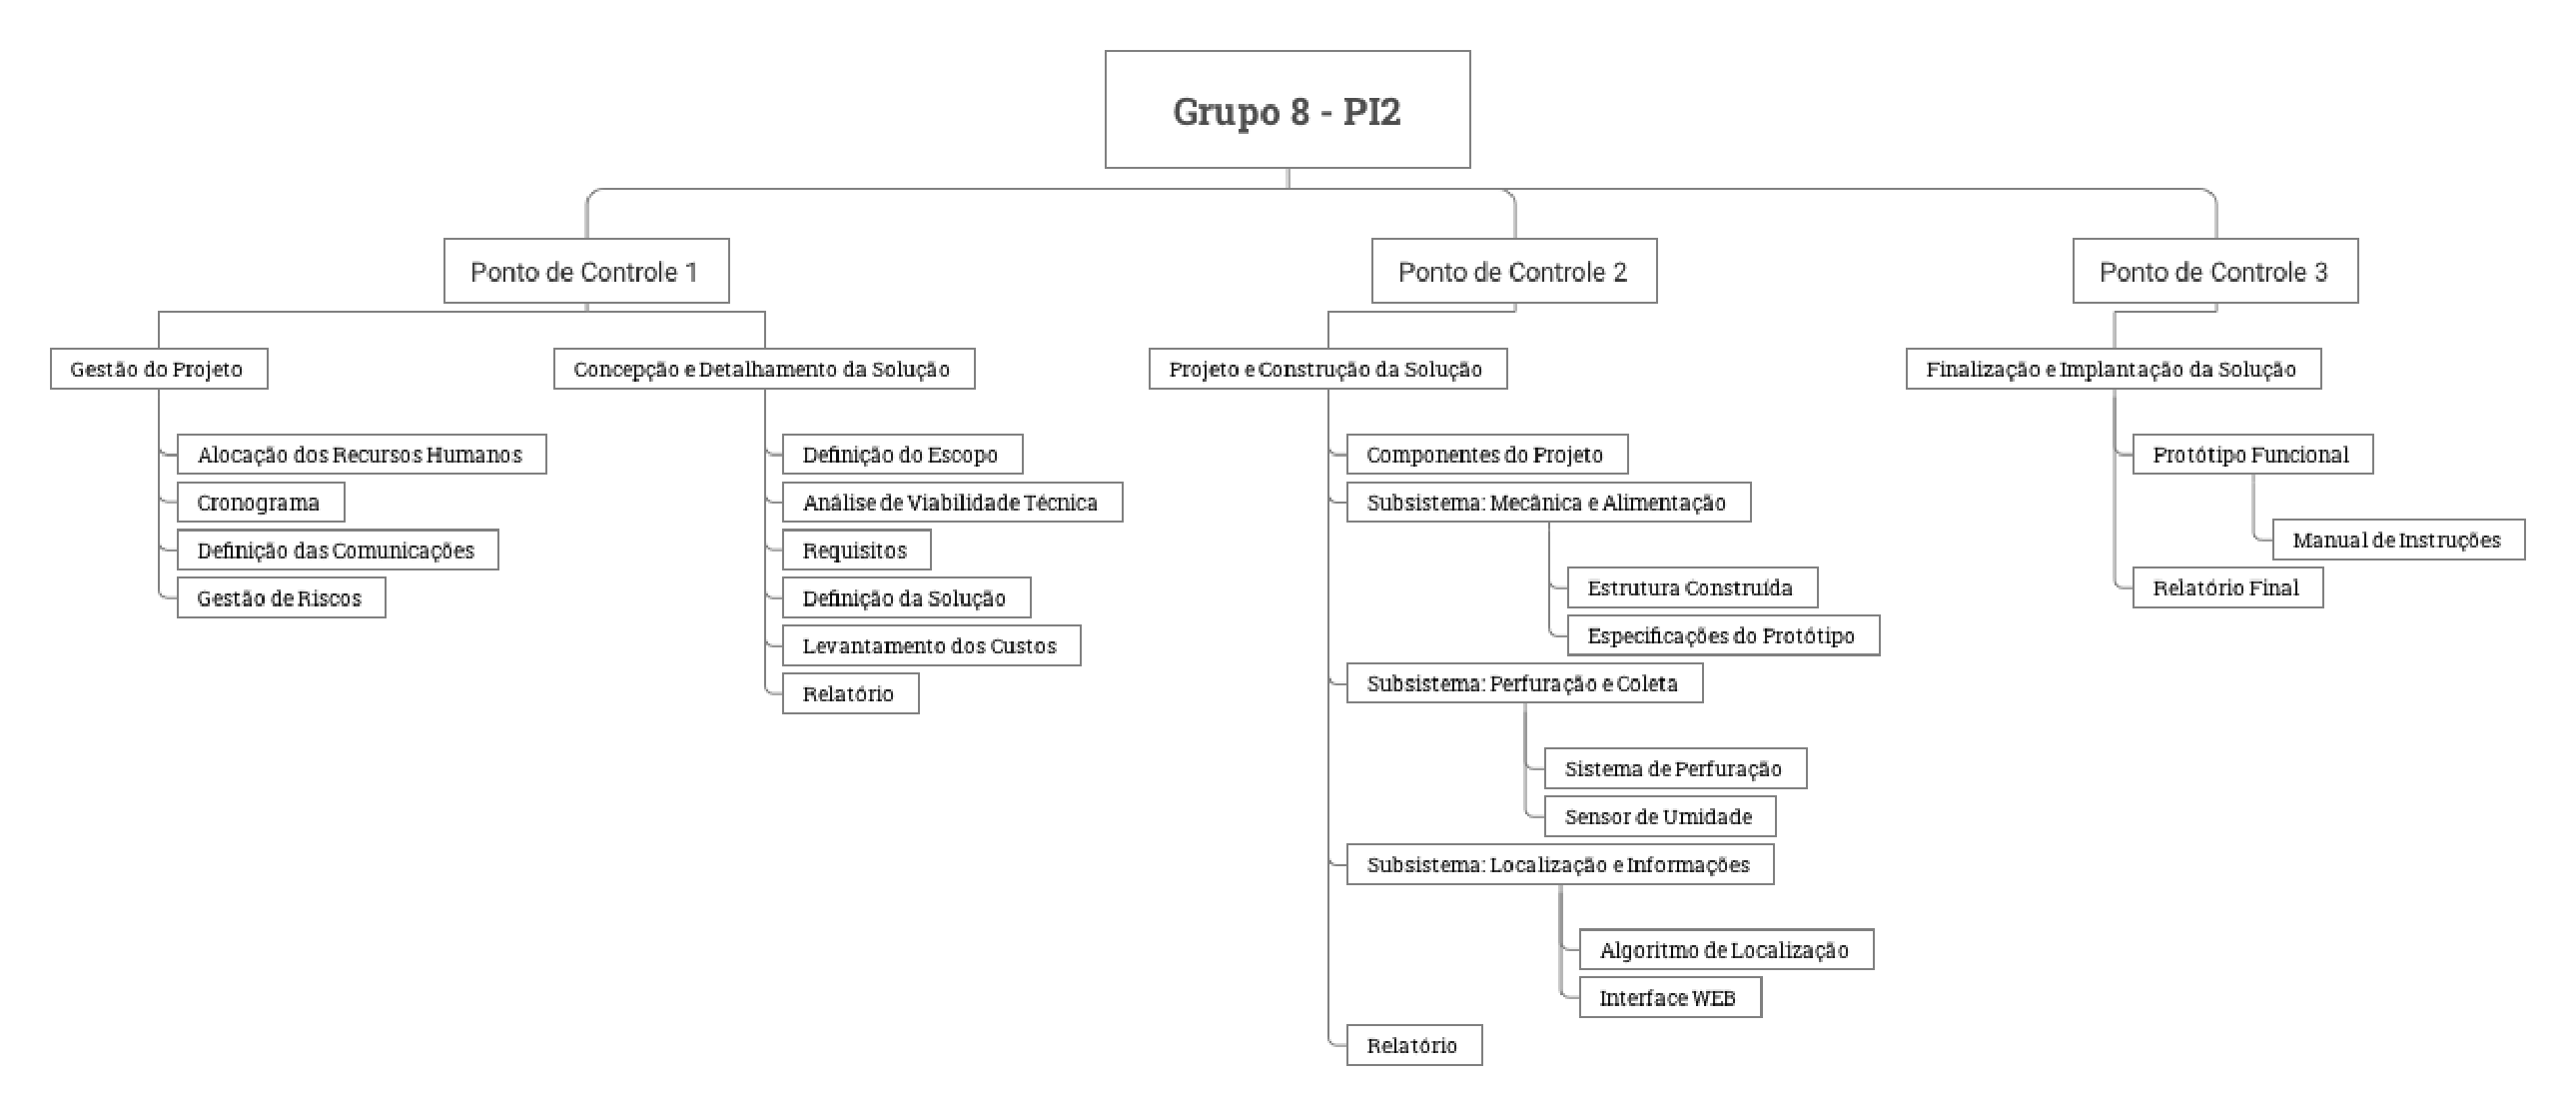
\includegraphics[width=\textwidth]{figuras/EAP.eps}
        \caption{Estrutura Analítica do Projeto. Fonte: autores.}
        \label{fig:eap}
      \end{figure}

      \vfill
      \pagebreak

    \subsection{Alocação dos Recursos Humanos}

      A equipe do projeto, formada por 15 (quinze) integrantes, foi
      subdivida em 3 (três) áreas de atuação, que são: "Mecânica e Alimentação", "Perfuração e Coleta" e "Localização e Informações".

      As áreas são supervisionadas e administradas por uma gestora geral, Jéssica Guimarães,
      e por um gestor da qualidade, Leonardo Cambraia.

      Cada uma das áreas citadas acimas é responsável pela análise de alternativas
      para a solução e a escolha de uma destas para ser aplicada no projeto.

      A figura \ref{fig:aloc} ilustra a estrutura de alocação de recursos humanos do
      projeto. A divisão dos integrantes foi feita levando em conta o
      interesse e conhecimento prévio individual nas áreas propostas.
      É importante salientar que toda a estrutura está sujeita a mudanças, sempre
      visando suprir as necessidades do projeto.

      \begin{figure}[!htbp]
        \centering
        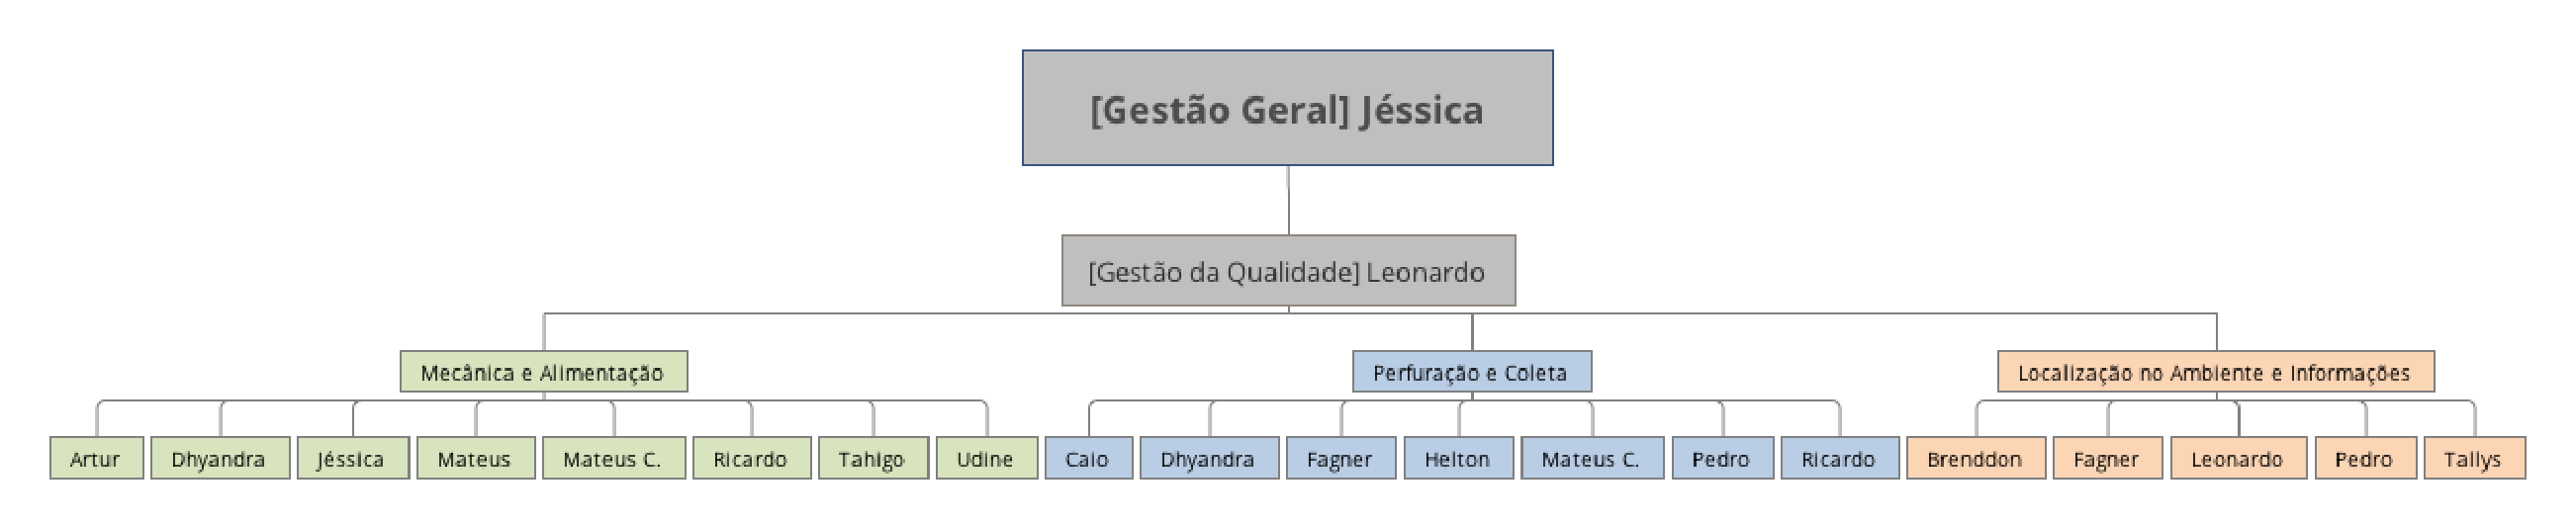
\includegraphics[width=\textwidth]{figuras/alocacao.eps}
        \caption{Alocação de recursos humanos. Fonte: autores.}
        \label{fig:aloc}
      \end{figure}

    \subsection{Comunicação}

      Para que qualquer projeto tenha sucesso é necessário o engajamento da equipe, sendo assim, é necessário uma comunicação eficaz entre os membros da equipe. A tabela \ref{tab:com} detalha os métodos de comunicação utilizados pela equipe.
      
      \begin{table}[!htbp]
      	\begin{center}
      		\caption{\label{tab:com}Métodos de comunicação. Fonte: autores.}
      		\begin{tabular}{|p{4cm}|p{4cm}|p{3cm}|p{3cm}|p{2cm}|}
      			\hline
      			\textbf{Objetivos} & \textbf{Ferramenta} & \textbf{Frequência} & \textbf{Horário} & \textbf{Local}\\\hline\hline
      			Acompanhamento das atividades & Kanban & Sob demanda & Horário da disciplina & FGA\\\hline
      			Avisos rápidos / Lembretes & Telegram & Sob demanda & N/A & N/A\\\hline
      			Decisões Técnicas/Planejamentos & Presencial & Duas vezes por semana & Horário da disciplina & FGA\\\hline
      			Desenvolvimento do projeto & Google Docs/ Google Hangouts/ Git / Github / Presencial & Sob demanda & Durante desenvolvimento do projeto & N/A\\\hline
      		\end{tabular}
      	\end{center}
      \end{table}

    \subsection{Tempo}

      Para a definição das atividades a serem realizadas durante o
      projeto utilizou-se como base os pacotes de trabalho estabelecidos
      na Estrutura Analítica do Projeto (EAP), onde os mesmos foram devidamente
      decompostos com base nos três grandes marcos do projeto referentes
      às entregas de Ponto de Controle 1, 2 e 3. Para tal feito, a equipe,
      tanto de gerência quanto de desenvolvimento precisará cumprir
      as atividades elucidadas no cronograma.

      Após decompostos os pacotes de trabalho da EAP, a equipe
      de gerência reuniu-se para discutir como suas atividades seriam
      executadas, visando tanto uma paralelização de atividades quanto
      o tempo estimado e os recursos necessários para tal.

      Para a determinação do tempo foram utilizadas as
      técnicas de \textbf{Analogia} e \textbf{Decisão em Grupo},
      as quais, segundo o \cite{PMI2012}, representam:

      \begin{itemize}
        \item Analogia: baseia-se em pacotes de trabalho/atividades similares
        de projetos anteriores para estimar a duração dos pacotes de trabalho
        e/ou atividades do seu projeto atual.
        \item Decisão em Grupo: nessa técnica o envolvimento da equipe de projeto
        nas estimativas proporcionam comprometimento da mesma com as
        atividades a serem realizadas.
      \end{itemize}

      O cronograma referente ao nosso projeto encontra-se na figura \ref{fig:cron_s1}
      e \ref{fig:cron_s2} abaixo, contendo seus pacotes de trabalho, atividades e datas. Outro
      cronograma mais detalhado está disposto no Apêndice \ref{schedule_ap}.

      \begin{figure}[!htbp]
        \centering
        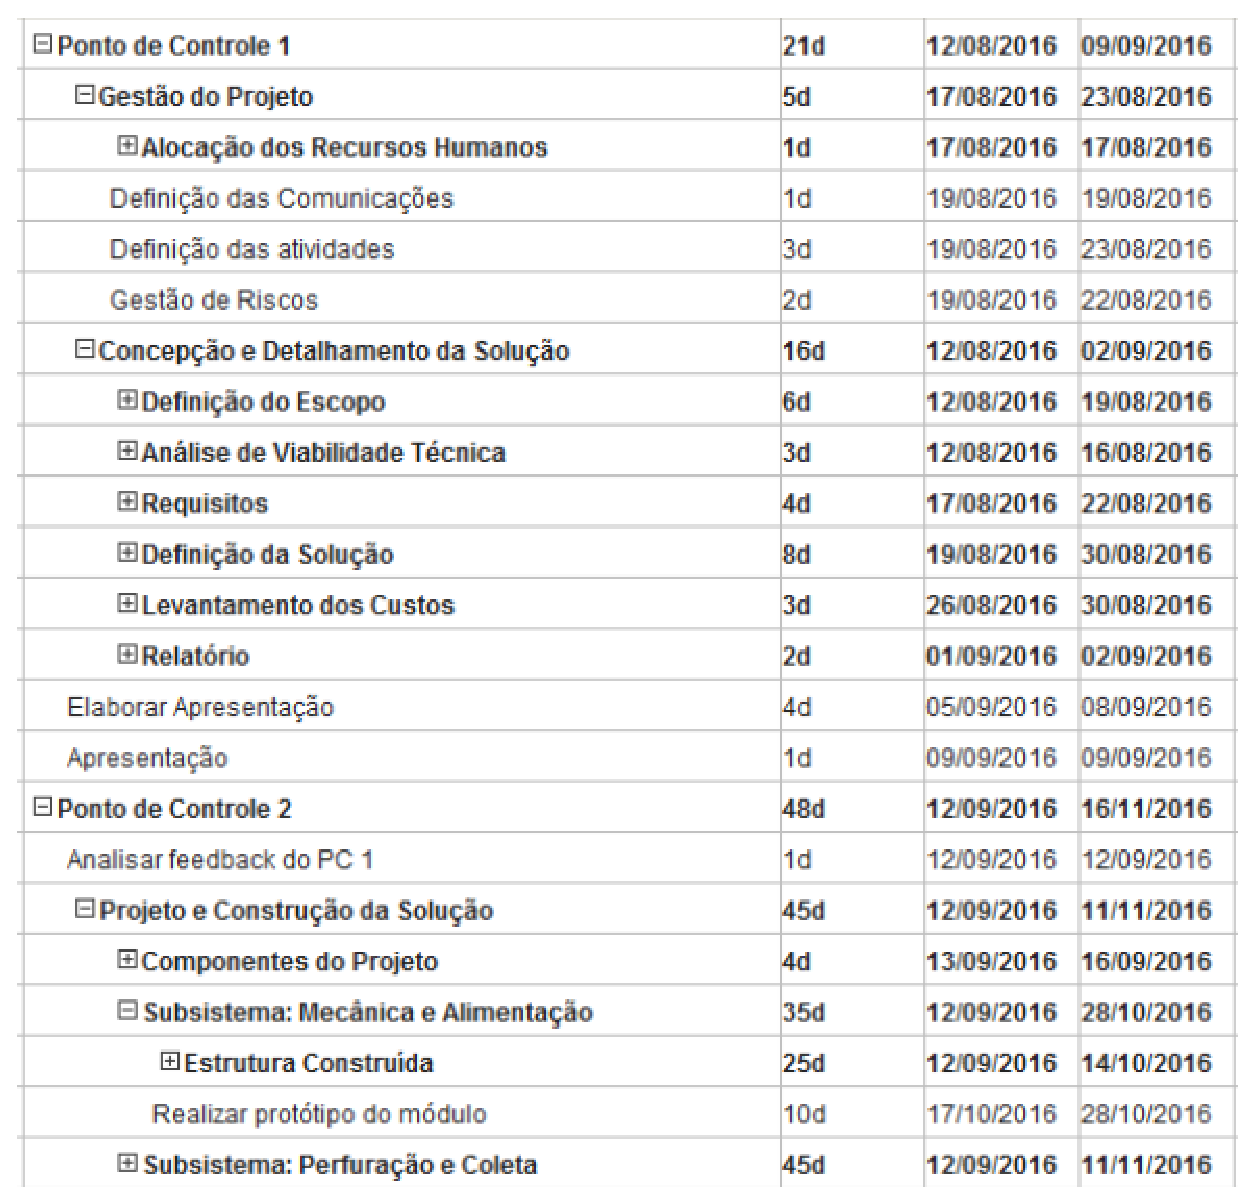
\includegraphics[width=\textwidth]{figuras/cronograma_simples_1.eps}
        \caption{Cronograma de Atividades simplificado (parte 1). Fonte: autores}
        \label{fig:cron_s1}
      \end{figure}

      \clearpage

      \begin{figure}[!htbp]
        \centering
        \includegraphics[width=\textwidth]{figuras/cronograma_simples_2.eps}
        \caption{Cronograma de Atividades simplificado (parte 2). Fonte: autores}
        \label{fig:cron_s2}
      \end{figure}

      \vfill
      \pagebreak


  \section{Riscos}

    A probabilidade e os impactos do riscos para o projeto classificam-se conforme a tabela abaixo:

  \begin{table}[!htbp]
    \begin{center}
    \caption{\label{probabilidadeximpacto}Relação Probabilidade x Impacto}
    \begin{tabular}{|l|l|l|}
    \hline
    \textbf{Probalidade} & \textbf{\% de certeza} & \textbf{Impacto} \\ \hline\hline
    Baixa                & 0 - 30                 & Pequeno          \\ \hline
    Média                & 31 - 60                & Regular          \\ \hline
    Alta                 & 61 - 100               & Alto             \\ \hline
    \end{tabular}
    \end{center}
  \end{table}

  O impacto dos riscos foram divididos em 3 níveis, onde:

  \begin{itemize}
    \item Pequeno: consiste em um risco que afetará pouco o projeto, sua ocorrência não deve interferir no cronograma ou no
    custo do projeto.
    \item Regular: consiste em um risco que afetará consideravelmente o andamento do projeto, podendo atrasar datas referentes
    aos sub-processos de um pacote de trabalho no cronograma, as quais refletirão diretamente no custo do projeto.
    \item Alto: consiste em um risco de alto impacto ao projeto, sua ocorrência pode atrasar entregas de um ponto de controle,
    comprometer completamente um pacote de trabalho ou até mesmo a interação entre a equipe. Estratégias de prevenção deverão
    ser realizadas imediatamente.
  \end{itemize}

  Para uma maior visualização do quão crítico pode ser um risco, realizou-se a Matriz de Probabilidade e Impacto:

  \begin{table}[!htbp]
    \begin{center}
    \caption{\label{impactoporprobabilidade}Relação Impacto / Probabilidade}
    \begin{tabular}{|l|l|l|l|}
    \hline
    \textbf{Impacto / Probabilidade} & \textbf{Baixa} & \textbf{Média} & \textbf{Alta} \\ \hline\hline
    Pequeno                          & Baixo          & Baixo          & Médio         \\ \hline
    Regular                          & Baixo          & Médio          & Alto          \\ \hline
    Alto                             & Médio          & Alto           & Alto          \\ \hline
    \end{tabular}
    \end{center}
  \end{table}

  Segundo \cite{scofanogestao}, as estratégias para resposta de ameaças à um projeto podem ser classificadas da seguinte maneira:

  \begin{itemize}
    \item Evitar: modificar o plano de projeto para eliminar o risco, a condição ou proteger os objetivos do projeto destes
    impactos. Mesmo sabendo que não existe a possibilidade de se eliminarem todos os eventos de risco, alguns riscos
    específicos, porém, podem ser evitados.
    \item Transferir: alterar a consequência de um risco para uma terceira parte juntamente com a responsabilidade de
    resposta. Essa estratégia não elimina o risco, apenas transfere sua responsabilidade para outra parte.
    \item Mitigar: reduzir a probabilidade e/ou consequências de um evento de risco adverso para um nível aceitável. Procura
    realizar ações preventivas para que não tenha consequências a serem reparadas.
    \item Aceitar: incluir um plano de contingência a ser executado quando da ocorrência de um. Esta técnica indica que a equipe
    não fará alterações no plano do projeto para negociar com um risco ou que não há resposta adequada.
  \end{itemize}

  Além das ameaças, também existem as estratégias para eventos que possam ser benéficos ao projeto, as quais são:

  \begin{itemize}
    \item Explorar: utilizar para riscos com impacto positivo, caso exista a necessidade de garantir a oportunidade pela organização.
    \item Compartilhar: alocar integral ou parcialmente a propriedade da oportunidade a um terceiro que detenha maior
    capacidade de gerir determinada oportunidade para benefício do projeto.
    \item Melhorar: empregar para aumento de probabilidade e/ou impactos positivos de uma possível oportunidade.
    \item Aceitar: aproveitar uma devida oportunidade sem que haja alocação de esforços dos recursos do projeto.
  \end{itemize}

  Para a identificação dos riscos foram realizados brainstormings entre a equipe, objetivando uma maior transparência
  e alertas sobre os riscos em si. Os riscos do projeto encontram-se na tabela \ref{tab:riscos}.

  \begin{table}[!htbp]
    \centering
    \caption{Riscos do projeto.}
    \label{tab:riscos}
    \resizebox{\textwidth}{!}{%
    \begin{tabular}{|p{3cm}|p{3cm}|p{3cm}|p{3cm}|p{3cm}|p{3cm}|p{3cm}|}
    \hline
    \textbf{Risco}                                      & \textbf{Efeito}                                                            & \textbf{Impacto} & \textbf{Probabilidade} & \textbf{Criticidade} & \textbf{Ação}                                                                                                                                        & \textbf{Estratégia} \\ \hline\hline
    Descompromisso de membros da equipe                 & Não cumprimento das atividades e sobrecarga sobre outros membros da equipe & Regular          & Média                  & Médio                & Conversar com o integrante e oferecer suporte para as dificuldades                                                                                   & Mitigar             \\ \hline
    Não cumprimento do cronograma                       & Valor de negócio será inferior ao planejado                                & Regular          & Média                  & Médio                & Ajustar cronograma para o trabalho que foi acumulado                                                                                                 & Mitigar             \\ \hline
    Erro na estimativa/planejamento do projeto          & Não entrega do produto no tempo previsto                                   & Grande           & Média                  & Alto                 & Reavaliar o escopo e redimensionar o projeto                                                                                                         & Mitigar             \\ \hline
    Necessidade de trabalhar mais horas que o planejado & Cansaço na equipe e redução na qualidade do produto                        & Regular          & Média                  & Médio                & Marcar reuniões com a sub-equipe para melhoria do desempenho                                                                                         & Aceitar             \\ \hline
    Inexperiência para a construção da solução          & Não conseguir entregar o produto e redução na qualidade do produto         & Regular          & Alta                   & Alto                 & Marcar reuniões com profissionais especialistas, alunos que já tiveram contato com a temática e procurar artigos acadêmicos relacionados ao assunto. & Mitigar             \\ \hline
    Integrante desistir da disciplina                   & Sobrecarga de trabalho aos outros integrantes                              & Médio            & Baixa                  & Baixo                & Redistribuir as tarefas do entregante pela equipe                                                                                                    & Aceitar             \\ \hline
    Requisitos se alterarem                             & Mudanças grandes no planejamento e estruturação do projeto                 & Grande           & Média                  & Alto                 & Replanejar o escopo do projeto                                                                                                                       & Mitigar             \\ \hline
    Danificação inesperada de componentes               & Não possuir material disponível para execução do projeto                   & Regular          & Baixa                  & Baixo                & Possuir componentes em estoque                                                                                                                       & Mitigar             \\ \hline
    Disponibilidade do local para testes                & Entregar o produto sem testes efetivos                                     & Grande           & Baixa                  & Médio                & Reservar o local com antecedência                                                                                                                    & Mitigar             \\ \hline
    Atraso na obtenção dos componentes                  & Atraso no cronograma e sobrecarga de trabalho                              & Grande           & Baixa                  & Médio                & Priorizar especificação e compra de componentes                                                                                                      & Mitigar             \\ \hline
    Integrantes com conhecimento além do esperado       & Impulsionamento da execução do projeto                                     & Grande           & Baixa                  & Médio                & Fazer com que o membro aplique e compartilhe bem o conhecimento                                                                                      & Explorar            \\ \hline
    \end{tabular}%
    }
  \end{table}
